
\subsubsection{WISE Research Group in Business Administration}

\paragraph{Research Team}

Sven Voelpel (Professor of Business Administration), Torsten Biemann (Postdoctoral Fellow; since 09/2007), Robert Eckhoff (Doctoral Fellow; since 10/2007), Polina Isichenko (Doctoral Fellow), Eric Kearney (Postdoctoral Fellow; since 10/2007), J�rg Korff (Doctoral Fellow; since 08/2007), Claudia Licklederer (Doctoral Fellow; since 07/2008), Daniela Noethen (Doctoral Fellow; since 04/2007), Anne Sauer (Doctoral Fellow; since 10/2008), Stefan Schaffer (Doctoral Fellow; since 11/2007), Katharina Speckmann (Doctoral Fellow; since 05/2008), Eden Tekie (Doctoral Fellow), Chunli Zhao (Doctoral Fellow).

%\newpage

\paragraph{}
Organizations must respond to a number of challenges brought about by major economic, technological, and demographic changes as well as heightened competition. There are many ways in which organizations can meet these challenges and gain competitive advantages. Generally, we examine the topics of wisdom, innovation, strategy, and energy in organizations. We investigate how the ongoing demographic changes and the rising average age in the workforce effect organizational outcomes in these domains (Voelpel, Leibold, \& Fr�chtenicht, 2007). Figure 16 provides an overview of these research efforts.

\paragraph{}
As a specific example of our research, we study how organizational teams should be composed to ensure high levels of performance and low levels of dysfunctional processes. In this regard, many authors view team heterogeneity (diversity) as a potential for increased creativity and innovation. Most importantly, we study under what conditions and through what processes age diversity can enhance team performance (Kearney, Voelpel, \& Gebert, 2008). 

\paragraph{}
\textit{Central Reference}

\paragraph{}
Voelpel, S., Leibold, M., \& Fr�chtenicht, J.-D. (2007). \textit{Herausforderung 50 plus: Konzepte zum Management der Aging Workforce: Die Antwort auf das demographische Dilemma.} Erlangen - New York: Publicis-Wiley (Vorwort von Heinrich von Pierer; Vorwort von Klaus Jacobs).

\paragraph{The WISE research domains are depicted in the following figure: }

\begin{figure}[htb]
  \begin{center}
    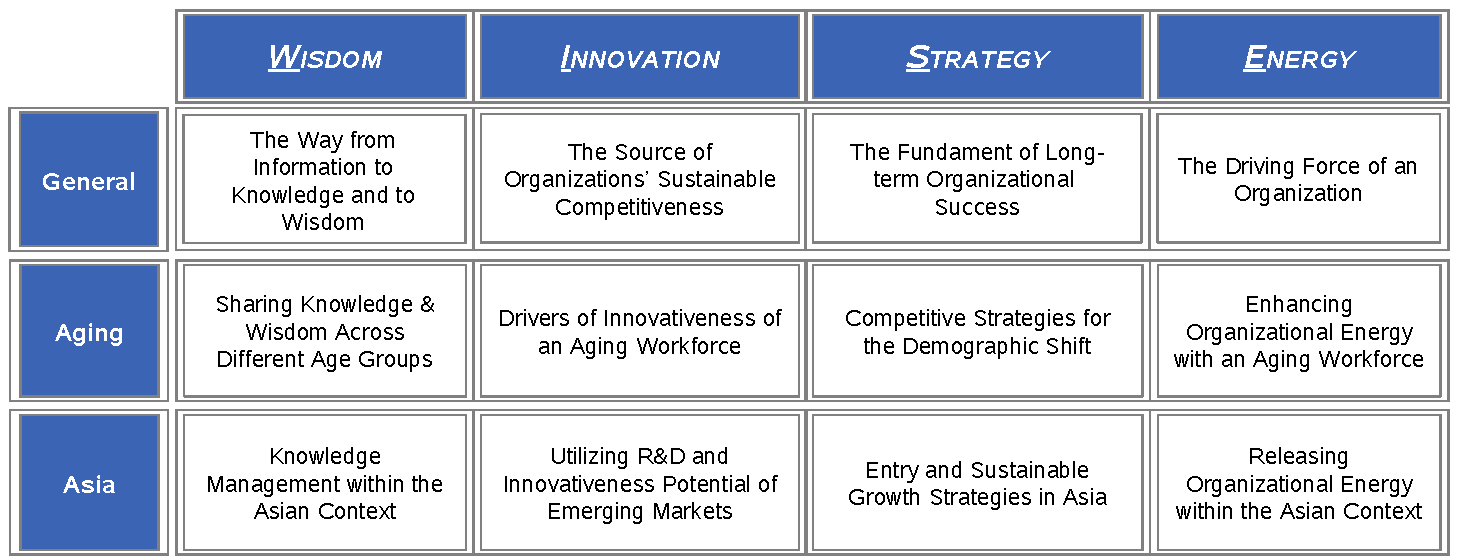
\includegraphics[width=0.5\textwidth,height=5cm]{profSvenVoelpel-fig1}
    \caption{Wise Research Domains }
    \label{fig1:profSvenVoelpel}
  \end{center}
\end{figure}

%\begin{flushleft}
%    \begin{tabular}{ | l | p{3cm} | p{3cm} | p{3cm} | p{3cm} |}
%    \hline
%        & \href{http://www.wiseresearch.org/index.php?do=wisdom}{WISDOM}  
%        & \href{http://www.wiseresearch.org/index.php?do=innov}{INNOVATION} 
%        & \href{http://www.wiseresearch.org/index.php?do=strategy}{STRATEGY} 
%        & \href{http://www.wiseresearch.org/index.php?do=energy}{ENERGY} \\ \hline
%    
%    GENERAL 
%    & \href{http://www.wiseresearch.org/index.php?do=wisdom}{The Way from Information to Knowledge and to Wisdom.}
%    & \href{http://www.wiseresearch.org/index.php?do=innov}{The Source of Organizations' Sustainable Competitiveness.}
%    & \href{http://www.wiseresearch.org/index.php?do=strategy}{The Foundation of Long-term Organizational Thrust.}
%    & \href{http://www.wiseresearch.org/index.php?do=energy}{The Driving Force of an Organization.} \\ \hline
    
%    AGING 
%    & \href{http://www.wiseresearch.org/index.php?do=energy}{Sharing Knowledge \& Wisdom Across Different Age Groups.} 
%    & \href{http://www.wiseresearch.org/index.php?do=innov&div=aging}{Drivers of Innovativeness of Aging Workforce.}
%    & \href{http://www.wiseresearch.org/index.php?do=strategy&div=aging}{Competitive Strategies for the Demographic Shift.}
%    & \href{http://www.wiseresearch.org/index.php?do=energy&div=aging}{Enhancing Organizational Energy with an Aging Workforce.} \\ \hline
    
%    ASIA 
%    & \href{http://www.wiseresearch.org/index.php?do=wisdom&div=asia}{Knowledge Management within the Asian Context. }
%    & \href{http://www.wiseresearch.org/index.php?do=innov&div=asia}{Utilizing R\&D and Innovativeness Potential of Emerging Markets.}
%    & \href{http://www.wiseresearch.org/index.php?do=strategy&div=asia}{Entry and Sustainable Growth Strategies in Asia. }
%    & RReleasing Organizational Energy within the Asian Context. \\ \hline
    
%    \end{tabular}

%\end{flushleft}

\subsubsection{WISE Demographic Network (WDN)}

\paragraph{Research Program}
On March 28$^{th}$ 2007, we founded the WISE Demographic Network (WDN) at the World Business Dialogue in Cologne. In times of demographic change, it is our objective to create strategic cooperation that aims to provide competitive advantages by enhancing innovation and productivity. Based on cooperation between academic research and organizations, practically applicable recommendations are formulated and tailored for individual organizations. Furthermore, it is intended that best practices and knowledge be exchanged. Another objective of the WISE Group is profiling an interdisciplinary research area. We have eight partner companies in the WDN:

\begin{itemize}

\item Daimler AG
\item Deutsche Bahn AG
\item Deutsche Bank AG
\item EnBW - Energie Baden-W�rttemberg AG
\item Lonza Ltd.
\item Mars GmbH
\item Otto GmbH \& Co. KG
\item Volkswagen AG

\end{itemize}

\paragraph{Research Highlights 2007/2008}
The WISE Demographic Network has conducted a qualitative analysis of its members' current status in terms of their demographic fitness. On the basis of a tailored focus group guideline, we identified the major fields of action of each member company. The analysis and comparison of the data of all member companies provided a solid basis for deriving various potential research strands. We have focused on three major issues that are of interest to all organizations: 

(1) Mechanisms, requirements, and obstacles of workplace learning;


(2) Employee organization amenable to achieving successful knowledge transfer (Teams)  and


(3) Age-differentiated application of HR practices (Talent Management). 

Three full-day WDN member conferences arranged in Bremen (October 07), Frankfurt (April 08), and Karlsruhe (October 08) helped to advance customized study efforts as well as best practice exchange.

\begin{figure}[htb]
  \begin{center}
    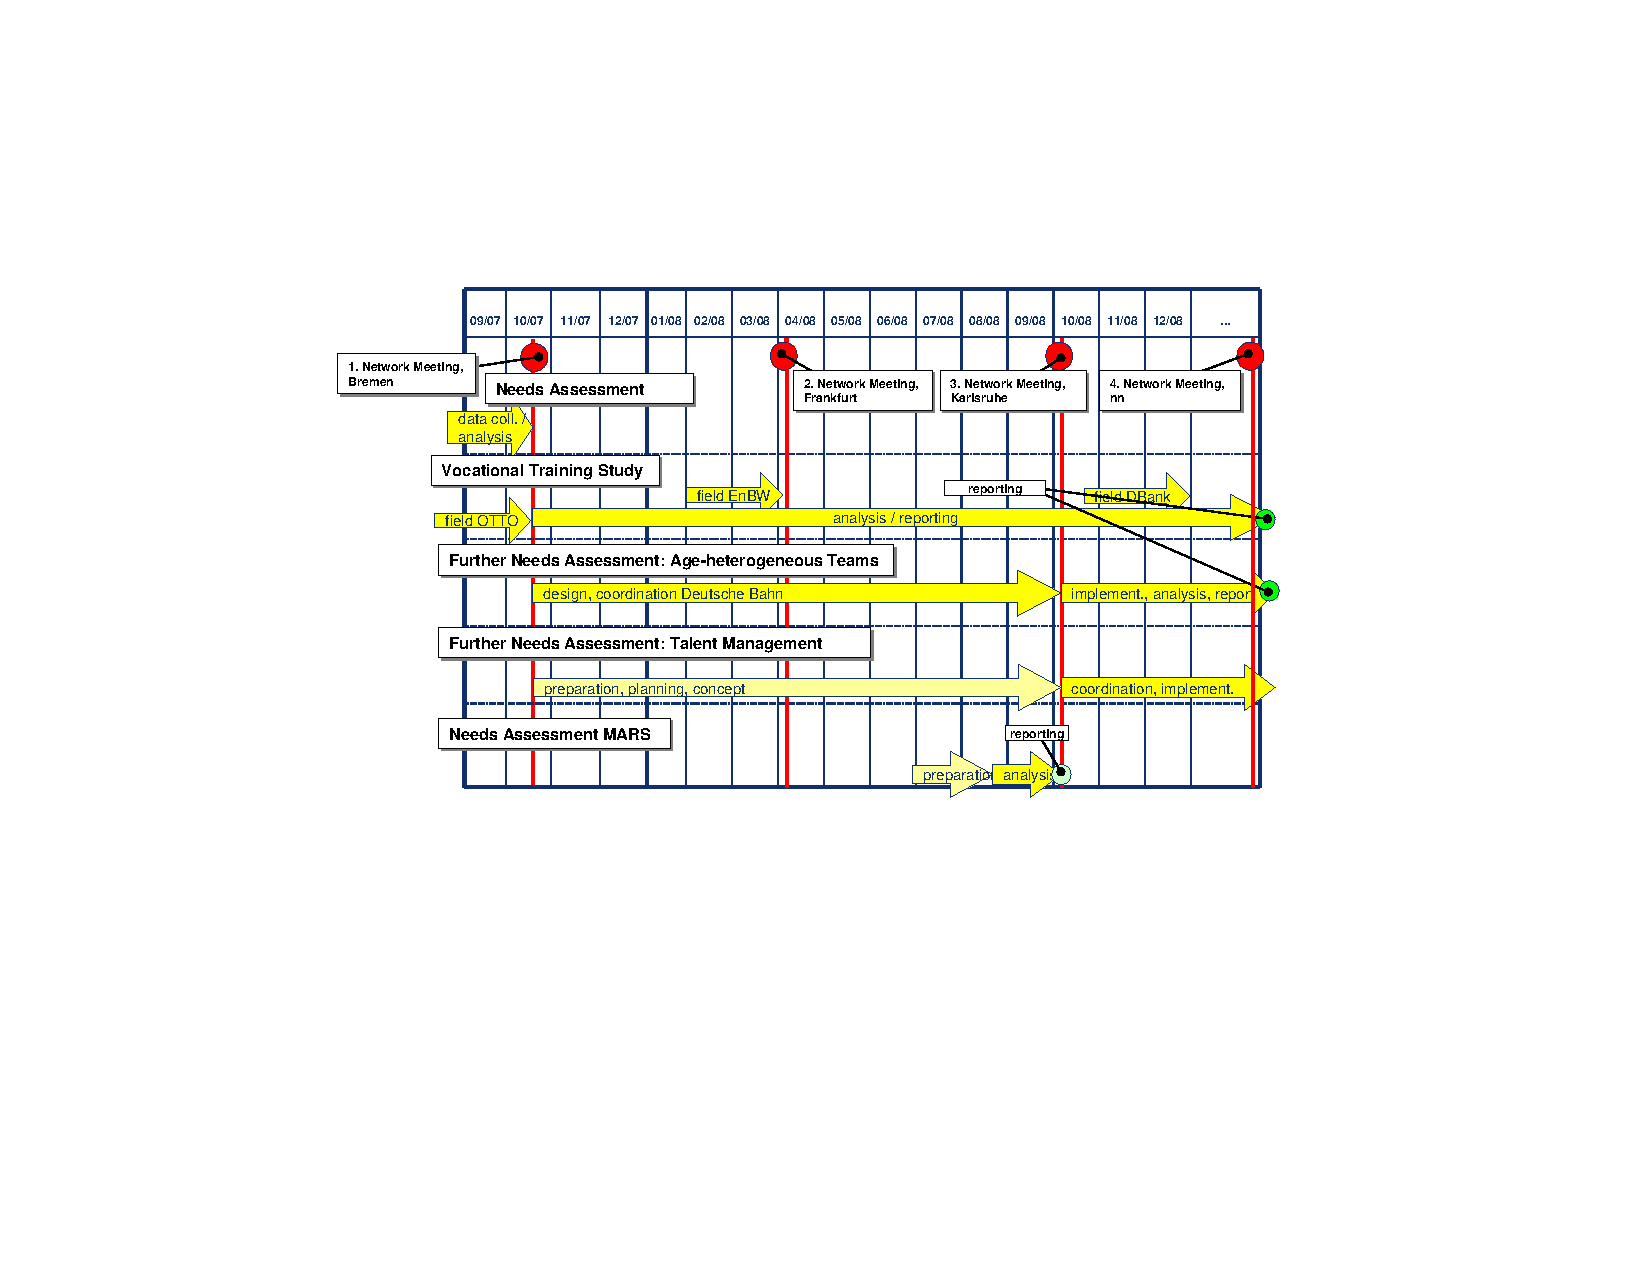
\includegraphics[width=0.5\textwidth,height=6.5cm]{Figure17_SV.pdf}
    \caption{WDN Activities.}
  \end{center}
\end{figure}


\subsubsection{Enhancing Aging Talents - Adjustment of Human Resource Management}

\paragraph{}

\begin{flushleft}
\textbf{Research Program}
\end{flushleft}


Research from strategic human resource management has provided sound evidence for the positive association between HR practices and organizationally valued performance (HRM-P). No theoretical framework has yet been provided, however, that is able to explain this relation.

\paragraph{}

\begin{flushleft}
\textbf{Research Highlights 2007/2008}
\end{flushleft}

In this project, an integrated HRM-P was developed that includes mediating variables that have been found empirically to be associated with organizational performance; these variables include (1) work motivation, (2) job satisfaction, and (3) organizational commitment (see Figure 18). The moderating role of employees' age for the mediated association was analyzed. The model aims to provide organizations with a basis on which to adjust their management tools in order to meet personnel challenges that have evolved due to demographic changes; this will permit employers and other relevant actors to preserve competitiveness.

\begin{figure}[htb]
  \begin{center}
    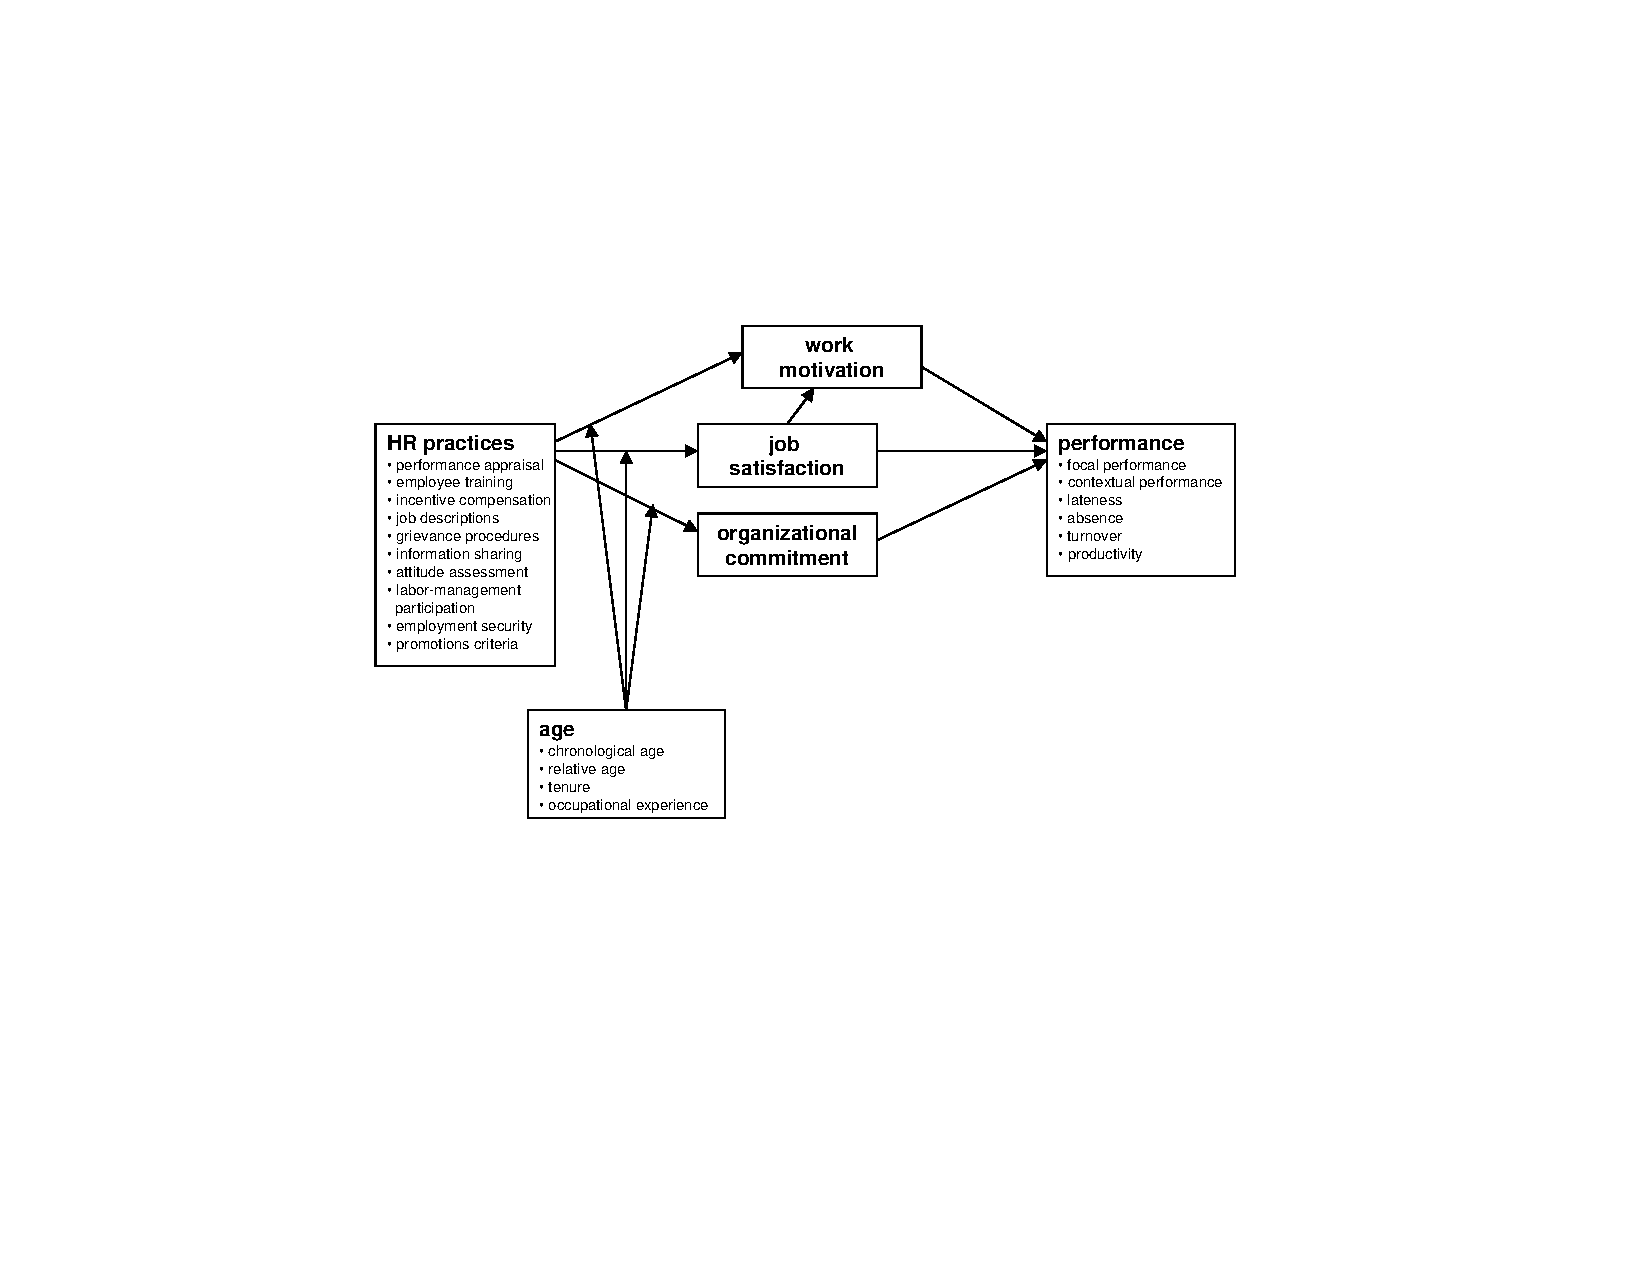
\includegraphics[width=0.5\textwidth,height=6.5cm]{Figure18_SV.pdf}
    \caption{Basic Research Model for the moderated and mediated relationship between HR practices and performance.}
    \label{Figure18_SV}
  \end{center}
\end{figure}

\paragraph{}
The model delineated above is primarily intended to be applied in the context of actual work settings. Taking this into account, we plan to gather empirical data by conducting surveys within various organizations. The project is currently acquiring organizations that are interested in participating in the empirical study.

\subsubsection{Knowledge Transfer: Demopass}

Analysing data from the interdisciplinary demopass-project (see 2.1), we are looking at influences on knowledge transfer within teams with a special focus on knowledge transfer between older (i.e. over 45 yrs.) and younger employees (i.e. under 30 yrs.). Moreover, we are investigating the connection between these types of knowledge transfer and performance. In terms of influences on knowledge transfer, we found a strong age effect with older employees engaging more in sharing knowledge with other team members while younger employees seek more knowledge from team members. In addition, employees in teams that have a lower average age in comparison to other teams seek more knowledge from team members. Furthermore, we found that extrinsic or intrinsic benefits motivate knowledge transfer within teams; while intrinsic benefits significantly influence individual knowledge sharing, extrinsic benefits motivate knowledge seeking. Finally, we found that high individual job autonomy encourages knowledge sharing while working in a team with high average job autonomy (compared to other teams) encourages individual knowledge seeking. Results on the connection between knowledge transfer and performance are forthcoming.

\subsubsection{Intergenerational Knowledge Transfer to Prevent Knowledge Loss in Organizations}

\paragraph{}

\begin{flushleft}
\textbf{Research Program}
\end{flushleft}

In the last decade, a knowledge-based perspective of the firm has emerged in strategic management literature. Knowledge is now seen as a resource that enhances productivity and conveys a competitive advantage for organizations. If older employees, with decades of experience, leave an organization, they take with them critical knowledge that they alone may possess, and whose loss leads to high costs for the organization. Although it has always been the case that employees retire and new employees are hired, this is especially problematic today because:

\begin{itemize}

\item Knowledge-intensive domains have become increasingly more specialized, complex and interdisciplinary;
\item Demographic changes, particularly waves of retiring baby boomers, have created new challenges; and
\item  Employees are now changing companies more often.

\end{itemize}

\paragraph{}

\begin{flushleft}
\textbf{Research Highlights 2007/2008}
\end{flushleft}

Several strategies have been proposed to prevent the costly loss of knowledge: they often involve, but are not limited to, HR processes, IT-tools, knowledge recovery initiatives, and knowledge transfer.
This project is focusing on the latter, proposing a coherent model of antecedents of knowledge transfer, as well as trying to establish a link between knowledge transfer between employees and the reduction of the threat of knowledge loss for an organization (see Figure 19). The objectives of this project can be summarized in three broad research questions:
\begin{enumerate}
	\item What are the main antecedents of knowledge sharing and knowledge seeking?
	\item Where does age play a role?
	\item Does knowledge transfer reduce the threat of knowledge loss?
\end{enumerate}

The project is currently in the phase of analyzing the empirical data. In addition, we intend to acquire additional organizations as collaboration partners.

%\begin{figure}[htb]
%  \begin{center}
%    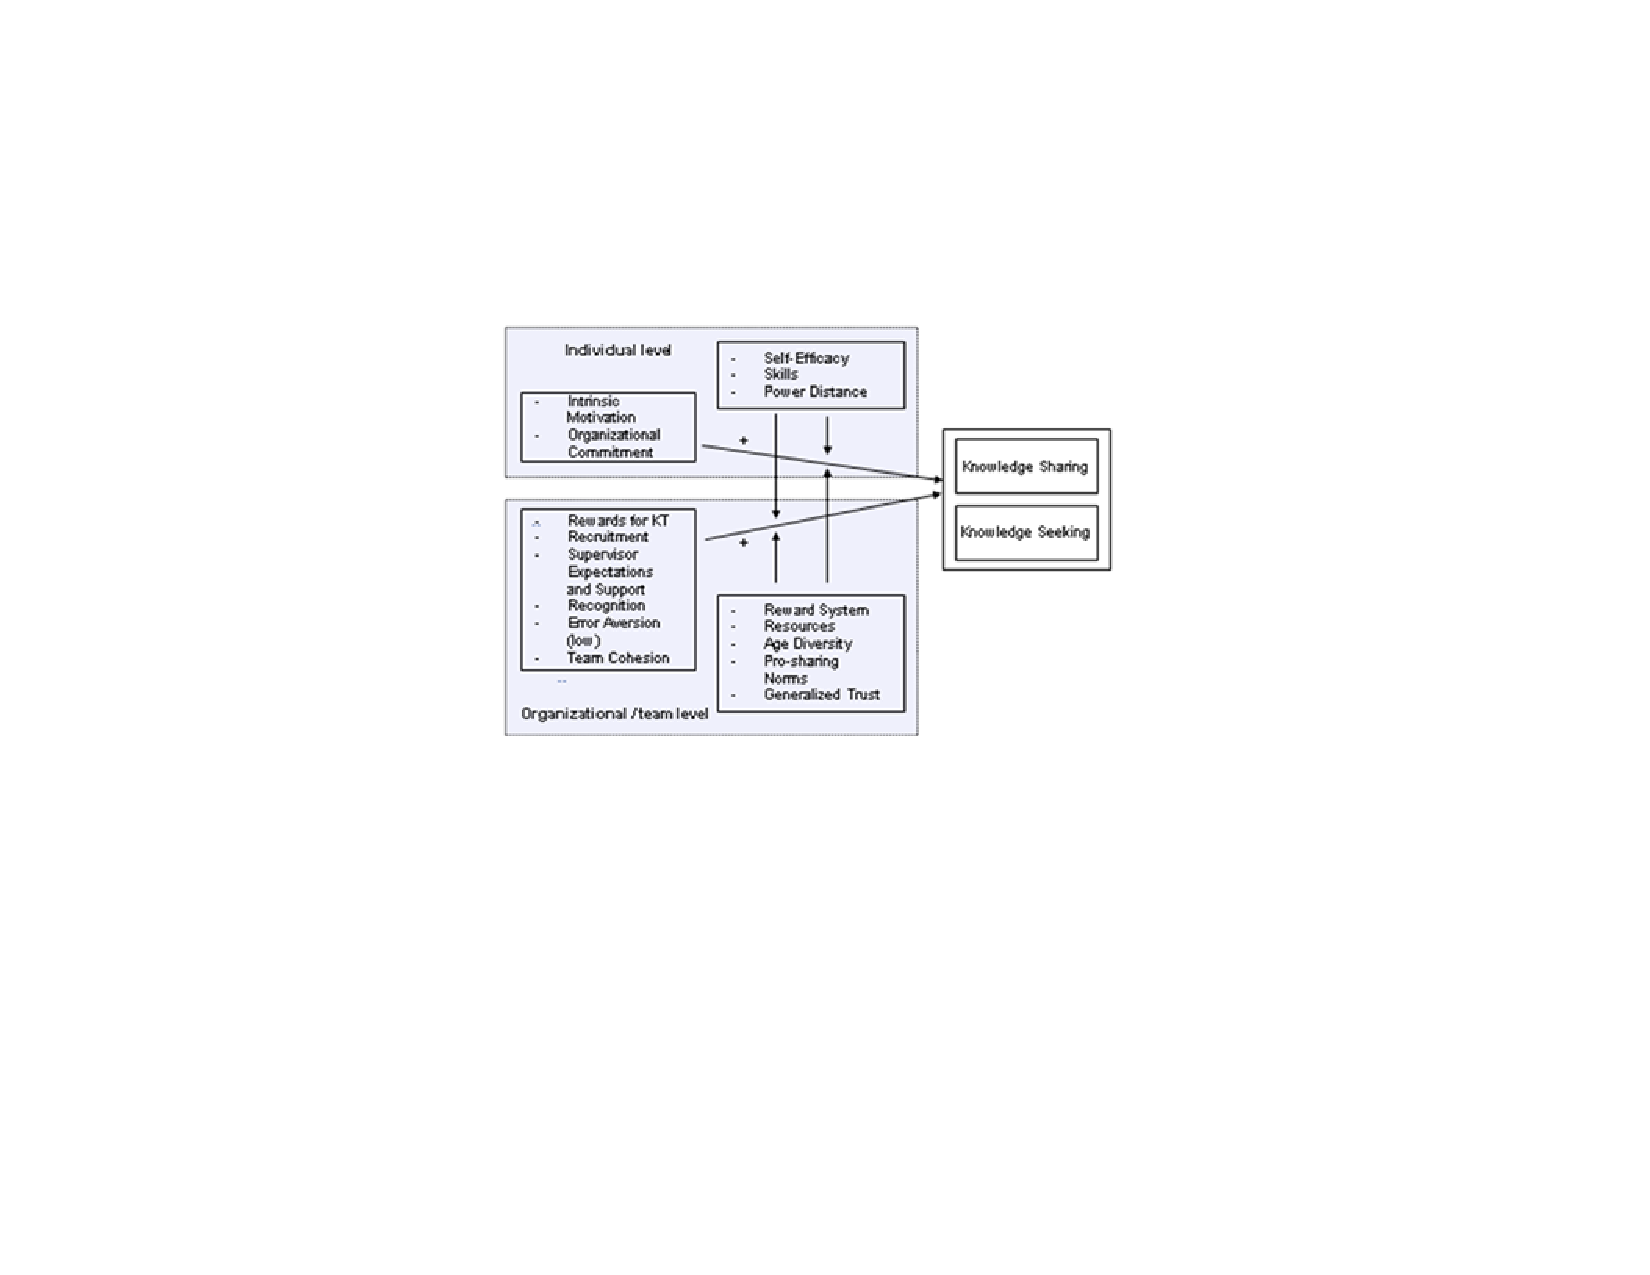
\includegraphics[width=0.5\textwidth,height=5cm]{Figure19_SV.pdf}
%    \caption{Basic research model on the antecedents of knowledge seeking and sharing.}
%  \end{center}
%\end{figure}

\paragraph{}
Within this broader framework of individual knowledge sharing in organizations, another focus is on knowledge exchange between different hierarchical levels, an aspect that very often also involves a difference in age. The objective of this empirical study is to investigate the decisive factors that influence employees' engagement in knowledge sharing with their supervisors.

\subsubsection{The Effects of the Aging Workforce on the Innovation Process: A Large-Scale Study of Technology Intensive Companies}

\begin{flushleft}
\textbf{Research Program}
\end{flushleft}

How will the aging of the workforce affect the innovativeness of organizations? The foundation of the innovation is ideas, and it is people who develop, carry, react to, and modify ideas. It is therefore important to recognize that innovation is based on individual and group performance efforts. As a result of the dramatic increase in the number of older employees in the workforces of developed industrial countries, the necessity to create innovation is more often than ever entrusted to aging employees. From this perspective, it is important to understand how this demographic trend changes individual and group behavior as it relates to innovation. 

\paragraph{}
Research has only recently begun to consider the relationship between the aging of workforces and the state of innovation processes. Unfortunately, this research has produced equivocal outcomes. We suggest that this is caused by: (a) a failure of the studies to include intervening processes that explain differences in innovative work behaviors across age cohorts; (b) a lack of distinction between radical and incremental idea-generation behaviors; (c) a paucity of empirical research on the relationship between aging and innovation in organizational settings; and (d) a neglect of the effects of increasing age diversity on group innovativeness. 

\paragraph{}
The goal of this research project is to overcome these knowledge gaps by developing a framework that explains the impacts of an aging workforce on innovation processes in organizational settings. This framework is meant to advance current knowledge in four important ways. First, it will connect aging to the behavioral activities involved in the innovation process through those factors that facilitate innovation. Innovative behavior across three behavioral activities will be analyzed: idea generation, innovation promotion, and implementation. Second, the framework will explore and explain the differences in idea generation patterns, innovation promotion, and implementation work behaviors across age cohorts. Understanding these differences will help us to draw possible conclusions about the implications of the aging of the workforce for organizational innovativeness. Third, it will explore and explain how innovation processes in workgroups are affected by an increase in those workgroups' age diversity. Finally, the framework will describe measures that enable organizations to intervene effectively into the relationship between aging and group innovation. Specifically, recommendations are expected to provide guidance for organizations on how to understand and benefit from innovative work behavior differences between younger and older-age cohorts across activity levels of the innovation process. They will also help companies integrate diverse innovative behaviors of age-dissimilar cohorts.

\paragraph{}
This project will collaborate with its industrial partner in order to access in-depth insights through interviews and surveys conducted in R\&D and technical teams of the company. The R\&D and innovation-related working groups of the industrial partner will serve as the units of analysis for quantitative and qualitative research.

\paragraph{}
Our study will employ a multi-method approach with a mix of quantitative and qualitative methods to generate and test our hypotheses. A concurrent triangulation strategy of the multi-method approach will be applied in order to confirm and cross-validate findings within a single study. The project will comprise a preparation phase, a study of mediators and moderators of the effect of age on the innovation behavior, a study of innovative behavior at individual and group levels, a comparative analysis, and a symposium.

\paragraph{}
We expect this project to generate a number of insights into this emerging and vibrant research topic, and to produce recommendations that will help organizations to improve the innovativeness of teams.

\subsubsection{Collaborations}

\begin{itemize} 
\item Massachusetts Institute of Technology, AgeLab, Prof. Dr. David DeLong 
\item Intellectual Capital Institute of Ireland, David O'Donnell 
\item Harvard Business School, Prof. Dorothy Leonard 
\item Babson College, Prof. Thomas H. Davenport 
\item ETH Zurich, Prof. Dr. Georg Von Krogh 
\item University of Stellenbosch, Prof. Marius Leibold 
\item Hitotsbashi University, Prof. Ikujiro Nonaka 
\item Wharton, Prof. Dr. Martine Haas 
\item Open University, Dr. J.C. Spender 
\item University of St. Gallen, Prof. Heike Bruch 
\item Erasmus University Rotterdam, Prof. Daan van Knippenberg 
\item Autonomous Universidad Madrid, Prof. Ramon Rico 
\item University of Groningen, Prof. Gerben van der Wegt 
\item University of Amsterdam, Prof. Dr. Astrid Homan 
\item Peking University, Prof. Dr. Max von Zedtwitz Gerben van der Wegt
\item Massachusetts Institute of Technology, Prof. Dr. Alan MacCormack 
\item Harvard University, Prof. Michael Beer 
\item University of California, Los Angeles, Prof. Barbara S. Lawrence 

\end{itemize}

\subsubsection{Publications}

\begin{itemize}
\item Voelpel, S., \& Kearney, E. (2008). Trust within organizations - Benefiting from demographic changes by fostering intra-organizational trust. \textit{Forum on Public Policy: Journal of the Oxford Roundtable}, 4(1): 1-17.

\item Kearney, E., Voelpel, S. C., \& Gebert, D. (2008). Examining the interaction of demographic diversity and personality - The role of need for cognition. \textit{Academy of Management Best Paper Proceedings}, 1-6. 
\item Voelpel, S., Eckhoff, R., \& F�rster, J. (2008). David against Goliath? Group size and bystander effects in virtual knowledge sharing. \textit{Human Relations}, 61(2): 273-297. 

\item Streb, C., Voelpel, S., \& Leibold, M. (2008). Managing the aging workforce: Status quo and implications for the advancement of theory and practice. \textit{European Management Journal}, 26(1): 1-10.

\item Han, Z., \& Voelpel, S. (2007). Knowledge Sharing in China: Reflections about Siemens' Experiences with ShareNet. \textit{Journal of Asian Business}, 23(1): 123-143.

\item Voelpel, S., \& Koch, J. (2008). Erfahrene Talente Bringen Weitblick. Fachteil: Demographischer Wandel. \textit{Personalwirtschaft}, 35(10): 44-46.

\item Voelpel, S., \& Koch, J. (2008). Zeitsammler und Talentj�ger. Fachteil: Demographischer Wandel in KMU. \textit{Personalwirtschaft}, 35(9): 46-49.

\item Voelpel, S., \& Koch, J. (2008). Wissen ist Marktstellung. Fachteil: Demographischer Wandel in KMU. \textit{Personalwirtschaft}, 35(8): 44-46.

\item Voelpel, S., \& Koch, J. (2008). Die passende Dosis finden. Fachteil: Demographischer Wandel in KMU. \textit{Personalwirtschaft}, 35(7): 46-48.

\item Voelpel, S., Koch, J. \& Afting, M. (2008). Wir sind DB. Gesichter, Stars und Hidden Champions: Das Talent Management der Deutschen Bahn wird als Kulturmanagement verstanden. \textit{Personal}, 60(7): 62-64.

\item Voelpel, S., \& Koch, J. (2008). Der Blick auf die St�rken. Fachteil: Demographischer Wandel. \textit{Personalwirtschaft}, 35(6): 44-46.

\item Voelpel, S., Koch, J., \& Korff, J. (2008). Die Gro�en im auf dem Weg zur demografischen Fitness. \textit{Personalwirtschaft}, 35(4): 44-46.

\item Ro�nagel, C., Picard, A.., \& Voelpel, S. (2008). Lernen jenseits der 40. \textit{Personal}, 60(4): 40-42.

\item Voelpel, S., \& Koch, J. (2008). Die neuen Davids. \textit{Personalwirtschaft}, 35(2): 49-51.

Otto, S., \& Voelpel, S. (2007). Demographischer Wandel in der Wirtschaft: Warum Unternehmen �ltere Arbeitnehmer brauchen. \textit{�kologisches Wirtschaften}, 26(4): 12-13.

\item Voelpel, S. (2007). Der Student als K�nig und Schwerstarbeiter. Eindr�cke von der Lehre an der Universit�t Harvard. \textit{Forschung \& Lehre}, 14(10): 598-600. 

\item Voelpel, S. (2007). Demografischer Wandel - Sage keiner, er sei nicht gewarnt worden. \textit{Personalwirtschaft}, 34(8): 18-22 (Comment by Wolfgang Clement, Chairman of the Adecco Institute). 

\item Rossnagel, C., \& Voelpel, S. (2007). Qualifizierung �lterer Mitarbeiter: Keine Einheitsweiterbildung. \textit{Persorama}, 31(1): 24-29. 

\item Voelpel, S., von Pierer, H., \& Streb, C. (2007). The mobile company: An integrated model for mobilizing to innovate. \textit{Profile}, 13, 59-65.

\item Staudinger, U. M., Ro�nagel, C. \& Voelpel, S. (2007). Personalmanagement und demographischer Wandel - eine interdisziplin�re Perspektive. In K. Schwuchow \& J. Gutmann, editors, \textit{Jahrbuch Personalentwicklung 2008 - Ausbildung, Weiterbildung, Management Development}�( 295-304). Munich/ Unterschlei�heim: Luchterhand.

\item Voelpel, S., Leibold, M., \& Fr�chtenicht, J.-D. (2007). H\textit{erausforderung 50 plus: Konzepte zum Management der Aging Workforce: Die Antwort auf das demographische Dilemma}. Erlangen - New York: Publicis-Wiley (Vorwort von Heinrich von Pierer; Vorwort von Klaus Jacobs). 

\end{itemize}